\chapter{Improving SUDS}

\section{Completing the implementation of UsernameToken}

As I mentioned in section \ref{sudsUsernameToken}, SUDS had an incomplete UsernameToken implementation that lacked complete digest support (it could be only set up manually), and even the plaintext method violated the standards by omitting the password type attribute. I changed the constructor of the \emph{UsernameToken} class in two ways.

\begin{itemize}
 \item A new parameter of boolean type called \emph{digest} was added to the parameter list. Its default value is set to \verb|False|, thus making it optional, so previously written code depending on this method will continue to work as expected.
 \item If the new parameter is missing or set to \verb|False|, the method performs the exact same instructions as before. But if it's set to \verb|True|, the \emph{nonce} and \emph{created} variables are set, and the \emph{digest} gets calculated according to the standard.
\end{itemize}

The \emph{xml} method -- which creates the actual tree of \emph{Element} objects -- was also modified, so that it sets the \emph{Type} attribute of the \emph{wsse:Password} element to the appropriate value, based on the \emph{digest} attribute. This change had the ``side effect'' that it made the plain text method standards compliant, so the \emph{UsernameToken} implementation of SUDS became complete and correct.

\section{Implementing digital signatures -- SudsSigner}

\subsection{Internal structure}

The internal structure of the plugin can be seen on Figure \ref{fig:cmpdSudsSigner}, the stereotypes describe the functionality (component or binding) and the runtime environment (Python or native) of each component. Native components are preferred for their reusability and performance -- reusable components are tested more thoroughly, as more projects can depend on them, which makes them less prone to errors, thus more suitable for security-critical tasks, such as cryptography (OpenSSL). From a performance point of view, XML parsing and processing is also a task that is better done using native and mature code (libxml2) because of its complexity. Python, on the other hand, is more suitable for the purpose of connecting components together, and describe high-level business logic in a readable and portable way.

\begin{figure}[htbp]
 \centering
 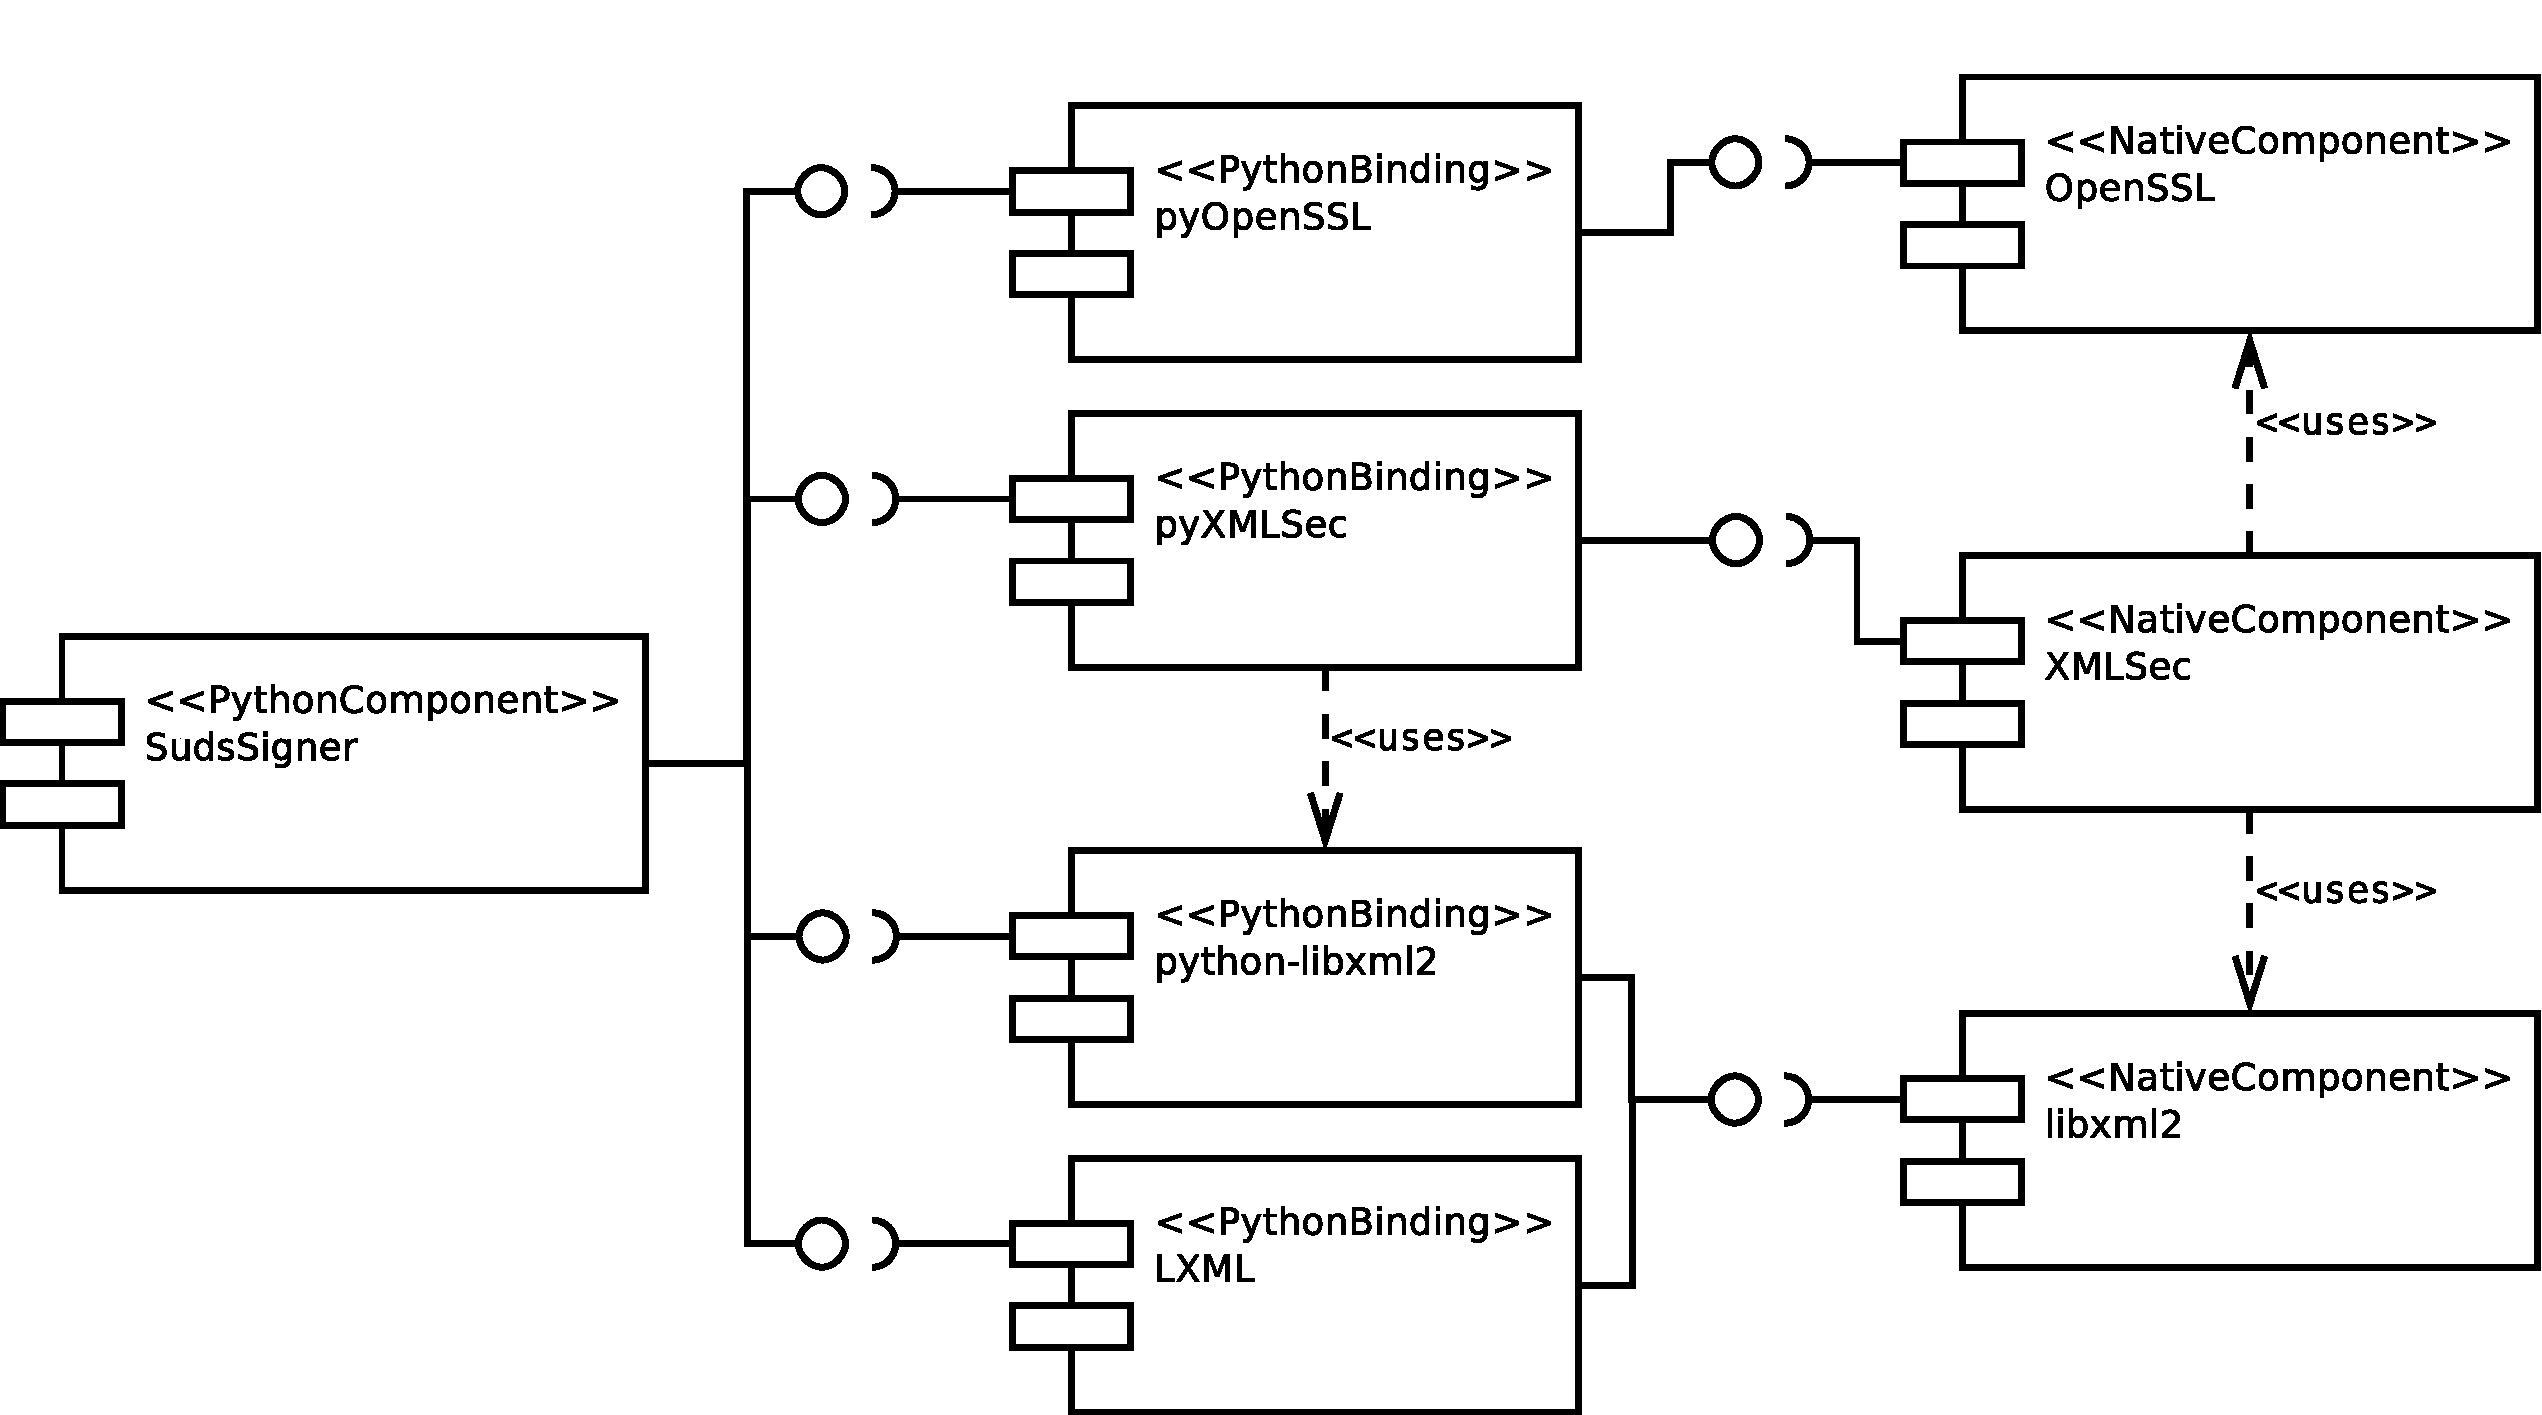
\includegraphics[width=\textwidth]{images/cmpdSudsSigner.pdf}
 \caption{Component diagram of the SudsSigner plugin}
 \label{fig:cmpdSudsSigner}
\end{figure}

\subsection{Components used}

\subsubsection{Libxml2, python-libxml2 and LXML}

``Libxml2 is the XML C parser and toolkit developed for the Gnome project (but usable outside of the Gnome platform), it is free software available under the MIT License.''\cite{libxml2-homepage} This sentence summarizes the project pretty well -- it's written in C, which is a good compromise between performance, portability and usability, and it's available under the MIT license, which makes it possible to either bundle it to FLOSS projects or redistribute it with proprietary software. Since many projects depend on it, the quality of the code is high, and it passes all of the OASIS XML Tests Suite.

\label{lxml}
Python-libxml2 provides low-level Python bindings to access all the functionality of libxml2. It has the advantages that the developer gets the full power of libxml2, but the interface resembles the original C API, which causes longer development and debug cycles. On the other hand, LXML\cite{lxml-homepage} wraps libxml2 in modules and classes providing a powerful high-level interface, which is more suitable for quick prototyping and maintainable codebase -- one good example of this difference is python-libxml2 returning error codes versus LXML throwing exceptions in erroneous situations.

I chose this combination because no other combination can offer the performance of the native parsing and processing engine combined with such rich and powerful Python interface.

\subsubsection{OpenSSL and pyOpenSSL}

``The OpenSSL Project is a collaborative effort to develop a robust, commercial-grade, full-featured, and Open Source toolkit implementing [\ldots] a full-strength general purpose cryptography library.''\cite{openssl-homepage} This library is also written in C, has a unique Apache and BSD-like license, and is FIPS 140-2 compliant. PyOpenSSL provides a friendly object-oriented interface, which makes it possible to access all the functionality of OpenSSL I needed. It's also well-maintained, which makes installing it on modern OSes a breeze. I chose this duo, because it seemed the only solution capable of handling PEM files in all the ways I needed.

\subsubsection{XMLSec and PyXMLSec}

XMLSec is a C library based on Libxml2 and supports XML signature, encryption and canonicalization.\cite{xmlsec-homepage} It's released under the MIT license, and is still maintained, so most Linux distributions provide it as an easily installable package. It uses libxml2 for XML processing and it can use several cryptography backends (OpenSSL, GnuTLS, Libgcrypt, NSS) for signature creation and encryption.

Python bindings were created for the Glasnost project financed by the French Department of Economy, Finance and Industry in 2003, but development seems to be ceased around 2005. The bindings are still working, only one feature needed a patch sent to the mailing list of the project in 2010. The documentation consists of a dozen examples and an API reference generated from the source code, so the use of these bindings require quite a bit of experimentation.

There are few other projects trying to create XML signatures, with not much success, so I chose this one, because at least it worked, and with a bit of work, I managed to make it do what I wanted.

\subsection{The Python component}

\begin{figure}[htbp]
 \centering
 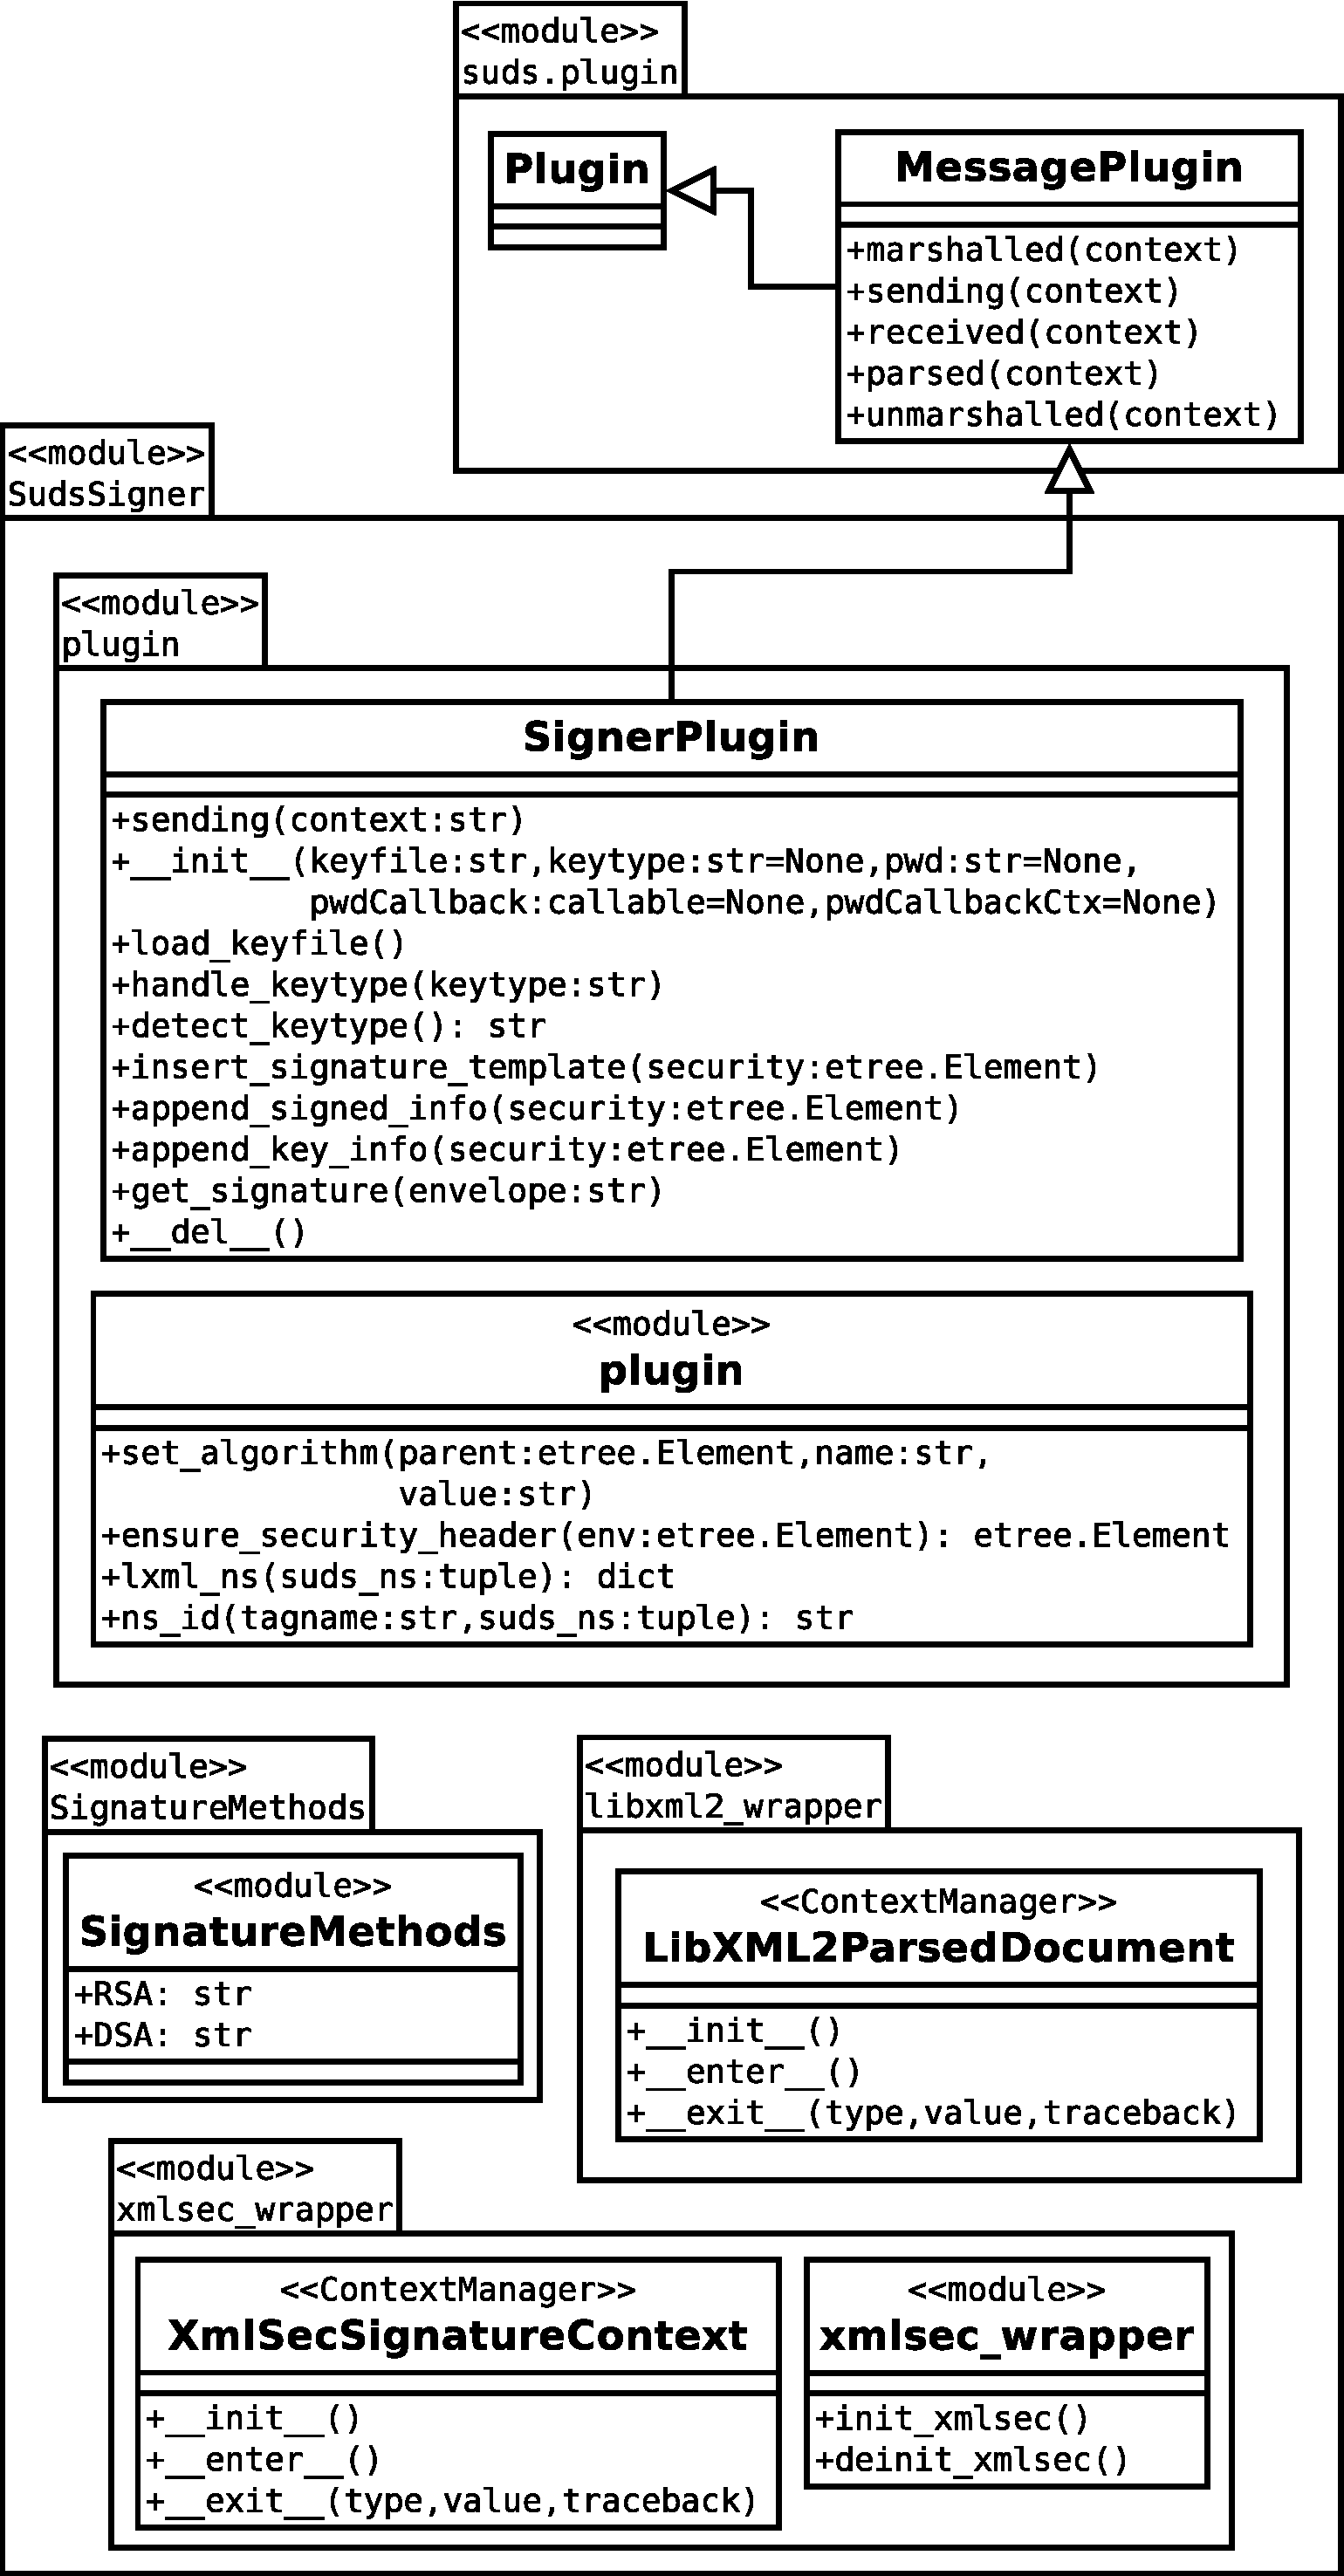
\includegraphics[height=22cm]{images/clsdSudsSigner.pdf}
 \caption{Class diagram of the SudsSigner Python component}
 \label{fig:clsdSudsSigner}
\end{figure}

The class diagram of the Python component of the plugin can be seen on Figure \ref{fig:clsdSudsSigner}, the Python-specific notations are expressed using stereotypes. Since UML doesn't support functions, just methods, each module with functions have a pseudoclass named after the module with \emph{module} stereotype. The main class is the \emph{SignerPlugin}, which directly interfaces SUDS, its \emph{sending} method is invoked after the SOAP envelope is complete, but before it's sent. The only parameter (\emph{context}) represents the SOAP invocation context, which makes the serialized envelope available through its \emph{envelope} attribute for access and modification. The method body is merely six lines of code, all elementary functionality is refactored to methods following the Single Responsibility Principle (SRP), and the functionality can be described as two distinct steps.

\begin{enumerate}
 \item The first step does two things -- first, it finds and marks the body of the SOAP envelope with an ID (currently constant \verb|suds-signed|), then the security header is selected (or created if necessary) and a so-called \emph{signature template} is inserted into it. This kind of processing is most easily done using the ElementTree implementation of LXML, therefore this part is framed with LXML parsing and serialization -- both the input and the output is an XML string.
 \item The second part finishes up and signs the XML output using the template provided with the XMLSec library. The input and output are XML strings again, this time parsed directly by the libxml2 parser.
\end{enumerate}

Although the performance of the Python component is affected by its interpreted runtime, I made several architectural decisions to rationalize CPU and memory consumption. The \emph{SudsSigner} class initializes the native libraries only once in the constructor and shuts them down in the destructor, thus reducing the time needed to process one single invocation. Native components need direct resource management because of the lack of garbage collection -- Python provides context managers for this problem, so I created two wrapper classes. \emph{LibXML2ParsedDocument} parses an XML string using python-libxml2, while \emph{XmlSecSignatureContext} encapsulates an XMLSec signature context object, and both free the resources upon leaving the scope of their use, thus minimizing memory usage.

\section{Testing and verification -- Arena}
\label{arena}

\subsection{Internal structure}

\begin{figure}[htbp]
 \centering
 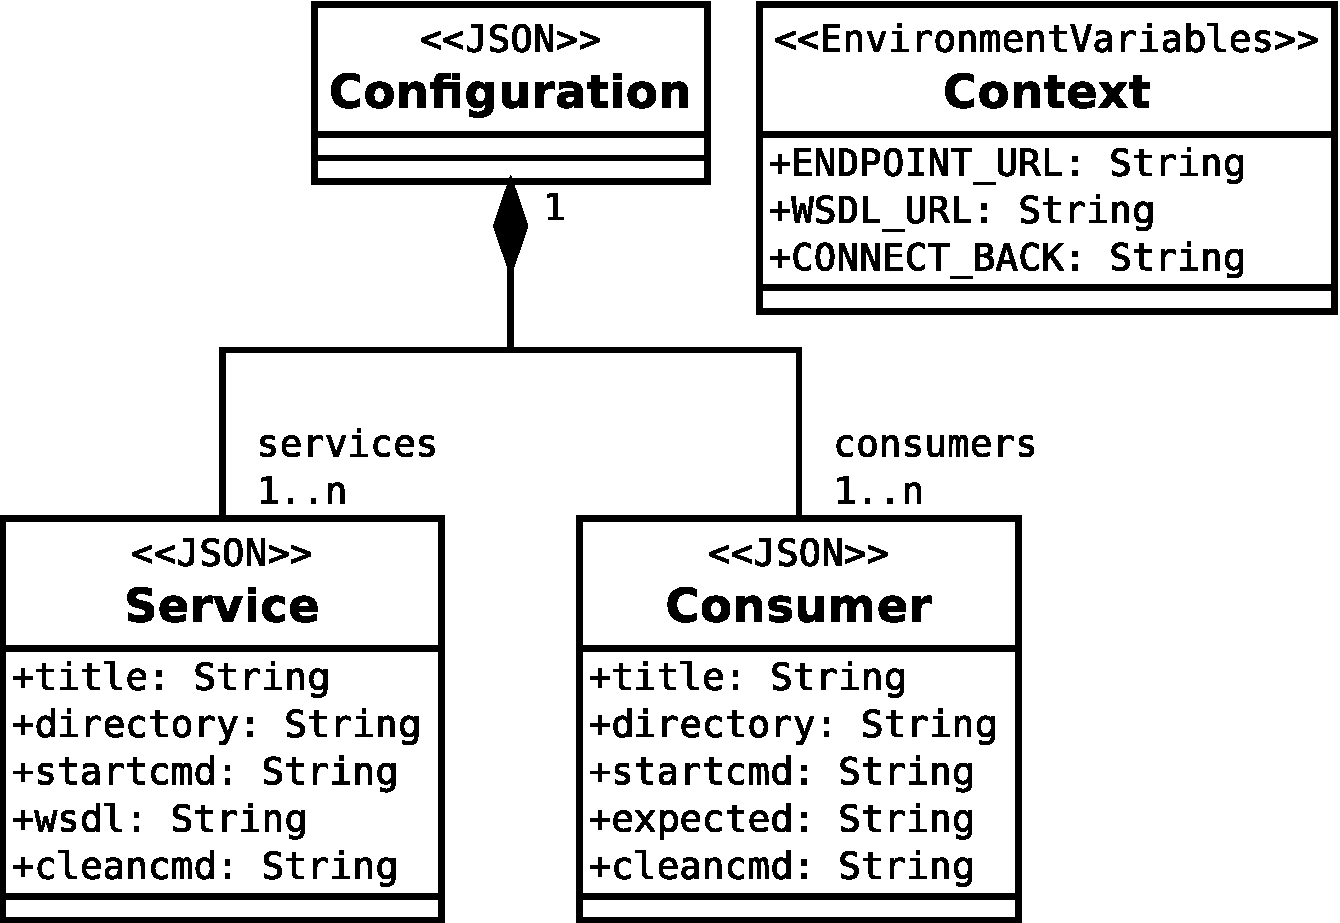
\includegraphics[width=11cm]{images/clsdArena.pdf}
 \caption{Class diagram of the business objects used in the \emph{Arena} testbed}
 \label{fig:clsdArena}
\end{figure}

Interoperability is one of the key motivations behind Service-Oriented Architecture, so a SOA component is essentially worthless without the capability of ``talking'' to other implementations. For this purpose, I developed a testbed called \emph{arena} before implementing any of the changes mentioned in the sections above. I chose Apache CXF as the reference implementation, although any solution could be plugged in easily. The registry of test subjects are stored in a JSON file (\verb|arena.json|) which contains a serialized \emph{Configuration} object (see class diagram on Figure \ref{fig:clsdArena}). Although the attribute names describe their intents, the following outline of processing should shed enough light on their usage to make the structure easy to understand.

\subsection{Outline of processing}

\subsubsection{Testing}
\label{arena_test}

Sample command line: \verb|python arena.py test cxf suds|

\begin{enumerate}
 \item The service named \emph{cxf} and the consumer named \emph{suds} are loaded from the registry.
 \item An unused TCP port number is generated using low-level socket operations.
 \item An endpoint URL is generated using the port selected in step 2 -- this gets stored in the environment value \verb|ENDPOINT_URL|.
 \item A TCP socket is created, and its availability (hostname and port separated with a colon) gets stored in the environment value \verb|CONNECT_BACK|.
 \item The WSDL URL is generated using the format provided in the \verb|wsdl| attribute of the service object. This URL gets stored in the environment value \verb|WSDL_URL|.
 \item The service gets started with its working directory set to the one specified in the \verb|directory| attribute of the service object.
 \item When the service is ready, it connects to the raw TCP socket specified in the \verb|CONNECT_BACK| environment value. The testbed waits for this connection using a -- currently hardcoded -- timeout.
 \item The consumer gets started just like the service, but with its stdout monitored by the testbed.
 \item The testbed waits for the consumer process to finish, and evaluates success based on the presence of the string specified in the \verb|expected| attribute of the consumer object on the standard output.
 \item Finally, the service process gets terminated, the testbed waits for it to finish up before exiting.
\end{enumerate}

\subsubsection{Cleaning}

Sample command line: \verb|python arena.py clean consumer cxf|

\begin{enumerate}
 \item The consumer named \emph{cxf} is loaded from the registry.
 \item If the \verb|cleancmd| attribute is specified, it gets executed in the directory specified in the \verb|directory| attribute of the service object.
\end{enumerate}

The cleaning process is important in case of solutions like Java, that use generated classes, which can cache previously used WSDL files referring to TCP ports that are no longer open.

\subsection{Generation of keys}

First, I used static keys from an earlier test, but later, the expired certificates cost me a lenghtful debugging session. To avoid this, I removed those keys, and created a small subsystem to generate the keypairs and certificates required for digital signature testing. Since Java -- and thus CXF, too -- prefers the Java Key Store (JKS) format, which nobody else really uses, one of my requirements was to create such solution that generates certificates along with private and public keys in both JKS and PEM formats. The direction of conversion is arbitrary, I chose generating the keypair in JKS, because the first working version used that, but it'd be trivial to change it to the opposite.

\begin{figure}[htbp]
 \centering
 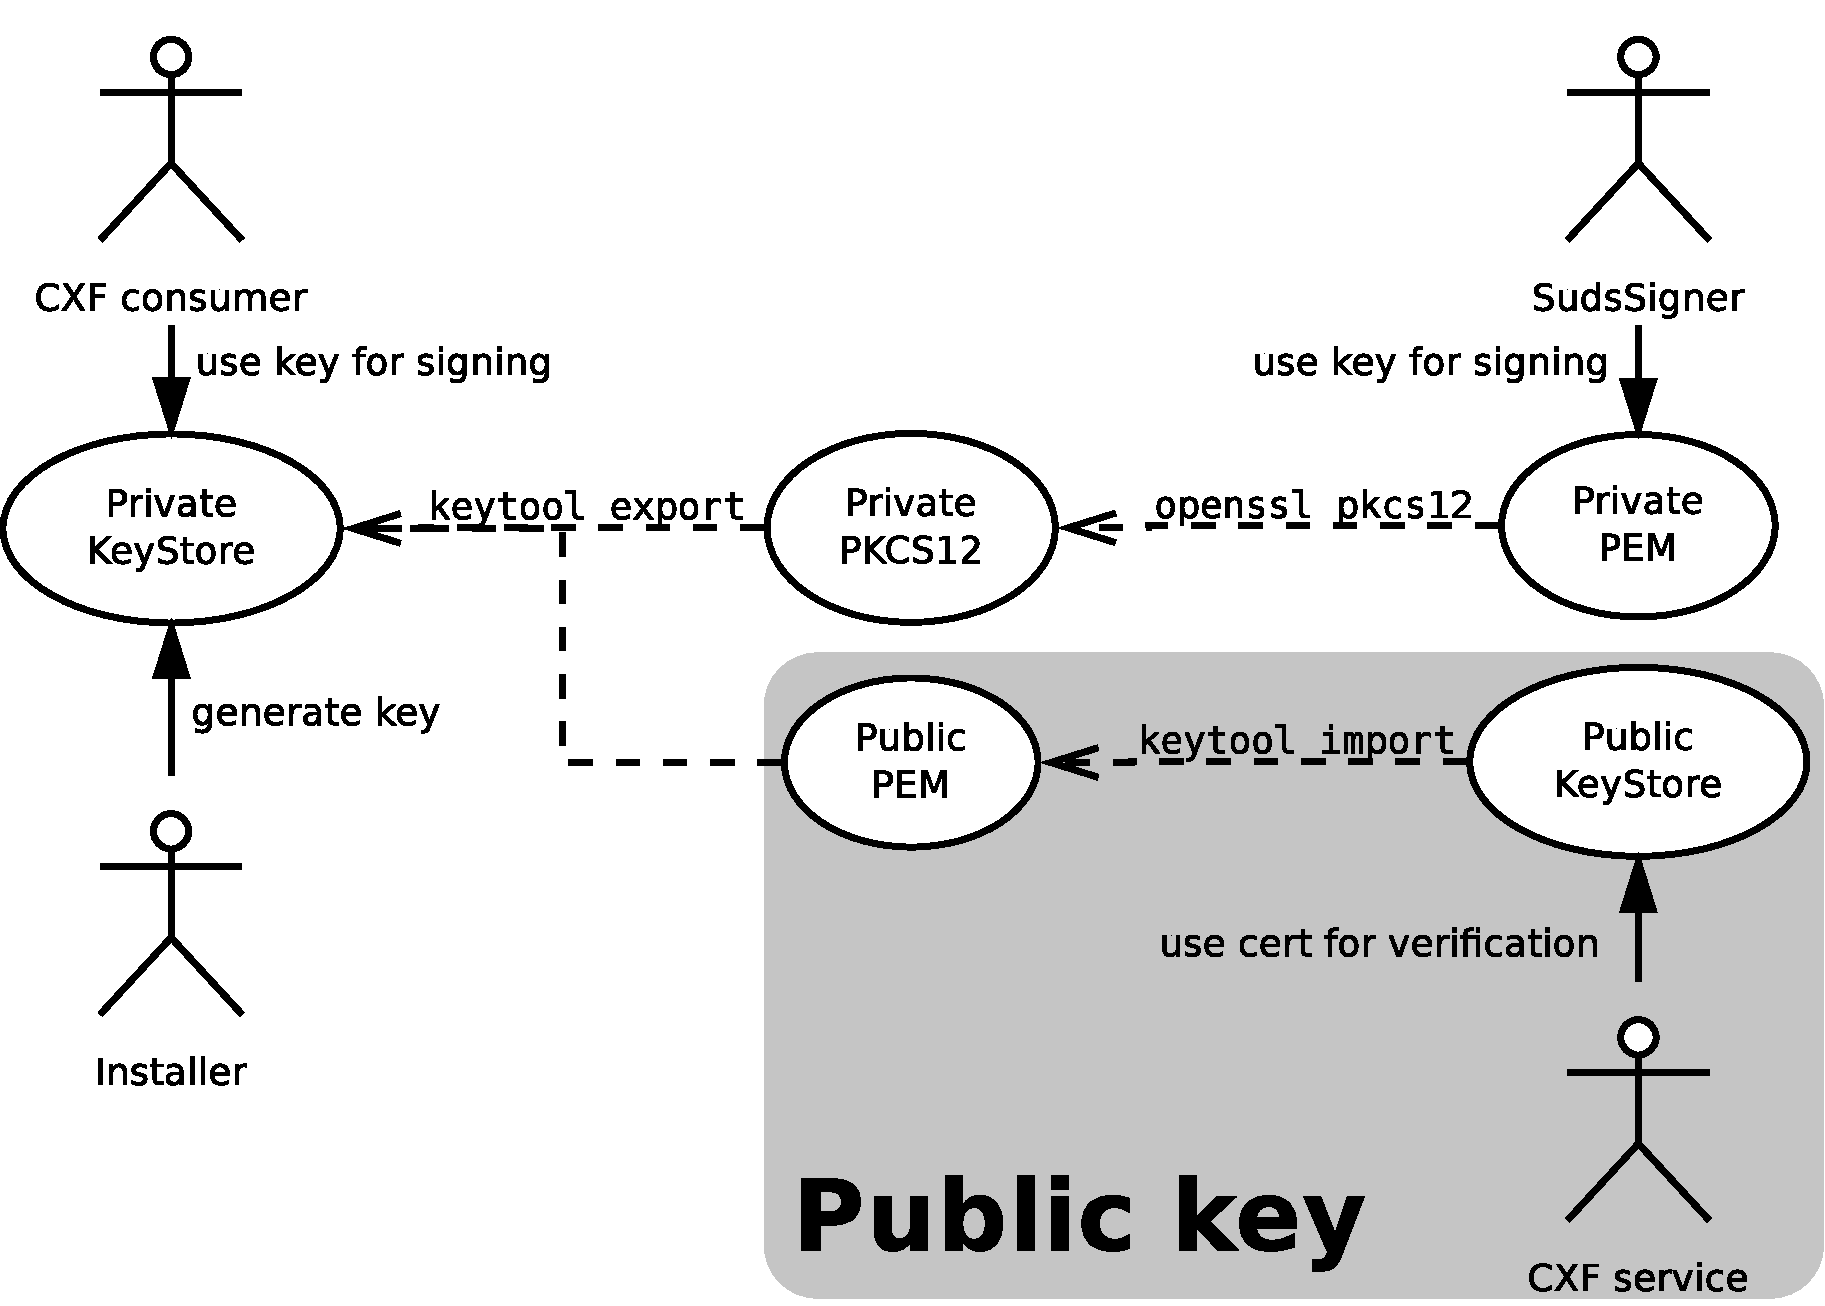
\includegraphics[width=14cm]{images/ucdArenaKeys.pdf}
 \caption{Use-case diagram of the \emph{Arena} testbed key generator}
 \label{fig:ucdArenaKeys}
\end{figure}

Since the generation and transformation of keys mainly consist of calling external programs (\emph{keytool} and \emph{openssl}) and involve dependency handling, \emph{make} was a logical choice. I implemented the use-cases and their dependencies (see Figure \ref{fig:ucdArenaKeys}) in a makefile, and by adding a pseudo target (\emph{phony} -- using the terms of \emph{make}) called \emph{all} as the first rule, which depends on the public KeyStore and the private PEM, issuing a \verb|make| command in the \verb|keys| directory of the testbed generates all the necessary keys in one step. All the dependency handling is automatically done by \emph{make}, if any key changes or goes missing, only the strictly necessary amount of files get regenerated -- but if necessary, the \emph{clean} pseudo target guarantees a fresh start.

\subsection{Usage during the development}

First, I created the testbed in parallel with developing a working CXF service-consumer pair. Besides easy development and testing, this setup made it trivial to capture network traffic generated by an already working solution -- something that made developing the SUDS improvements far more trivial than using just the specifications. I also changed a bit of the architecture later, as the first version used polling -- it tried connecting to the service in a tight loop, and started the consumer right after the first success. As it turned out, not all services are ready at the moment of socket binding, so I changed it to a push-style communication -- the service signals the testbed, when it's ready to receive consumer connections, which is also more resource conservative, since it requires one single TCP connection as opposed to lots of rejected polling packets.
